% !Mode:: "TeX:UTF-8"
% Author: Zhengxi Tian
% Email: zhengxi.tian@hotmail.com

\chapter{各指标在不同数据集和模型上的概率分布}
\label{ch:metric_dist}
我们在这里展示了指标的句子层面得分在不同数据集和模型的组合上的概率分布。
为了方便对比,我们把一个指标的分布画在一张矩阵图中,
矩阵的每一行的模型相同,每一列的数据集相同。
从这些图像中,我们可以同时在数据集和模型的维度观察句子层面得分分布
的变化规律。
一个主要的现象是,不同模型在相同数据集上具有相似的句子层面得分分布,
同一个模型在不同数据集上的句子层面得分分布差异较大。
这个现象再次说明了数据集对指标得分的影响比模型大。

% -- ADEM -- %
\begin{figure}[H]%
\centering%
\includegraphics[width=0.8\textwidth]{/home/cgsdfc/Metrics/Eval/data/v2/plot/distplot_grid/adem/plot.pdf}%
\caption{ADEM 的概率分布图}%
\label{fig:ADEMdist}%
\end{figure}

% -- BLEU -- %
\begin{figure}[H]%
\centering%
\includegraphics[width=0.6\textwidth]{/home/cgsdfc/Metrics/Eval/data/v2/plot/distplot_grid/bleu_1/plot.pdf}%
\caption{BLEU{-}1 的概率分布图}%
\label{fig:BLEU{-}1dist}%
\end{figure}
\begin{figure}[H]%
\centering%
\includegraphics[width=0.6\textwidth]{/home/cgsdfc/Metrics/Eval/data/v2/plot/distplot_grid/bleu_2/plot.pdf}%
\caption{BLEU{-}2 的概率分布图}%
\label{fig:BLEU{-}2dist}%
\end{figure}
\begin{figure}[H]%
\centering%
\includegraphics[width=0.8\textwidth]{/home/cgsdfc/Metrics/Eval/data/v2/plot/distplot_grid/bleu_3/plot.pdf}%
\caption{BLEU{-}3 的概率分布图}%
\label{fig:BLEU{-}3dist}%
\end{figure}
\begin{figure}[H]%
\centering%
\includegraphics[width=0.6\textwidth]{/home/cgsdfc/Metrics/Eval/data/v2/plot/distplot_grid/bleu_4/plot.pdf}%
\caption{BLEU{-}4 的概率分布图}%
\label{fig:BLEU{-}4dist}%
\end{figure}

% -- EB -- %
\begin{figure}[H]%
\centering%
\includegraphics[width=0.6\textwidth]{/home/cgsdfc/Metrics/Eval/data/v2/plot/distplot_grid/embedding_based_greedy_matching/plot.pdf}%
\caption{Greedy 的概率分布图}%
\label{fig:Greedydist}%
\end{figure}
\begin{figure}[H]%
\centering%
\includegraphics[width=0.8\textwidth]{/home/cgsdfc/Metrics/Eval/data/v2/plot/distplot_grid/embedding_based_vector_average/plot.pdf}%
\caption{Average 的概率分布图}%
\label{fig:Averagedist}%
\end{figure}
\begin{figure}[H]%
\centering%
\includegraphics[width=0.6\textwidth]{/home/cgsdfc/Metrics/Eval/data/v2/plot/distplot_grid/embedding_based_vector_extrema/plot.pdf}%
\caption{Extrema 的概率分布图}%
\label{fig:Extremadist}%
\end{figure}

% -- METEOR -- %
\begin{figure}[H]%
\centering%
\includegraphics[width=0.8\textwidth]{/home/cgsdfc/Metrics/Eval/data/v2/plot/distplot_grid/meteor/plot.pdf}%
\caption{METEOR 的概率分布图}%
\label{fig:METEORdist}%
\end{figure}

% -- Distinct-N -- %
\begin{figure}[H]%
\centering%
\includegraphics[width=0.8\textwidth]{/home/cgsdfc/Metrics/Eval/data/v2/plot/distplot_grid/distinct_1/plot.pdf}%
\caption{Distinct{-}1 的概率分布图}%
\label{fig:Distinct{-}1dist}%
\end{figure}
\begin{figure}[H]%
\centering%
\includegraphics[width=0.8\textwidth]{/home/cgsdfc/Metrics/Eval/data/v2/plot/distplot_grid/distinct_2/plot.pdf}%
\caption{Distinct{-}2 的概率分布图}%
\label{fig:Distinct{-}2dist}%
\end{figure}

% -- ROUGE -- %
\begin{figure}[H]%
\centering%
\includegraphics[width=0.6\textwidth]{/home/cgsdfc/Metrics/Eval/data/v2/plot/distplot_grid/rouge_1/plot.pdf}%
\caption{ROUGE{-}1 的概率分布图}%
\label{fig:ROUGE{-}1dist}%
\end{figure}
\begin{figure}[H]%
\centering%
\includegraphics[width=0.8\textwidth]{/home/cgsdfc/Metrics/Eval/data/v2/plot/distplot_grid/rouge_2/plot.pdf}%
\caption{ROUGE{-}2 的概率分布图}%
\label{fig:ROUGE{-}2dist}%
\end{figure}
\begin{figure}[H]%
\centering%
\includegraphics[width=0.8\textwidth]{/home/cgsdfc/Metrics/Eval/data/v2/plot/distplot_grid/rouge_3/plot.pdf}%
\caption{ROUGE{-}3 的概率分布图}%
\label{fig:ROUGE{-}3dist}%
\end{figure}
\begin{figure}[H]%
\centering%
\includegraphics[width=0.8\textwidth]{/home/cgsdfc/Metrics/Eval/data/v2/plot/distplot_grid/rouge_4/plot.pdf}%
\caption{ROUGE{-}4 的概率分布图}%
\label{fig:ROUGE{-}4dist}%
\end{figure}
\begin{figure}[H]%
\centering%
\includegraphics[width=0.6\textwidth]{/home/cgsdfc/Metrics/Eval/data/v2/plot/distplot_grid/rouge_l/plot.pdf}%
\caption{ROUGE{-}L 的概率分布图}%
\label{fig:ROUGE{-}Ldist}%
\end{figure}
\begin{figure}[H]%
\centering%
\includegraphics[width=0.6\textwidth]{/home/cgsdfc/Metrics/Eval/data/v2/plot/distplot_grid/rouge_w/plot.pdf}%
\caption{ROUGE{-}W 的概率分布图}%
\label{fig:ROUGE{-}Wdist}%
\end{figure}

% -- #words -- %
\begin{figure}[H]%
\centering%
\includegraphics[width=0.6\textwidth]{/home/cgsdfc/Metrics/Eval/data/v2/plot/distplot_grid/utterance_len/plot.pdf}%
\caption{\#words 的概率分布图}%
\label{fig:wordsdist}%
\end{figure}
